\chapter{Результаты и их сравнительный анализ} \label{ch4}

% не рекомендуется использовать отдельную section <<введение>> после лета 2020 года
%\section{Введение} \label{ch4:intro}

	Для измерения производительности предлагаемого конвейера, было разработано приложение, поддерживающее динамическое переключение конвейера вывода. При помощи данного приложения была создана тестовая сцена, на которой были проведены эксперименты. Данная сцена представляет собой помещение, в котром находится аквариум и единственный источник света (генерирующий тень), находящийся над аквариумом. В аквариуме находятся рыбы, каждая из которых имеет уникальные геометрию и материал. С течением времени, количество рыб в аквариуме увеличивается. Примеры работы представлены на \firef{fig:empty_aquarium} и \firef{fig:full_aquarium}.
	
	\begin{figure}[ht!] 
		\center
		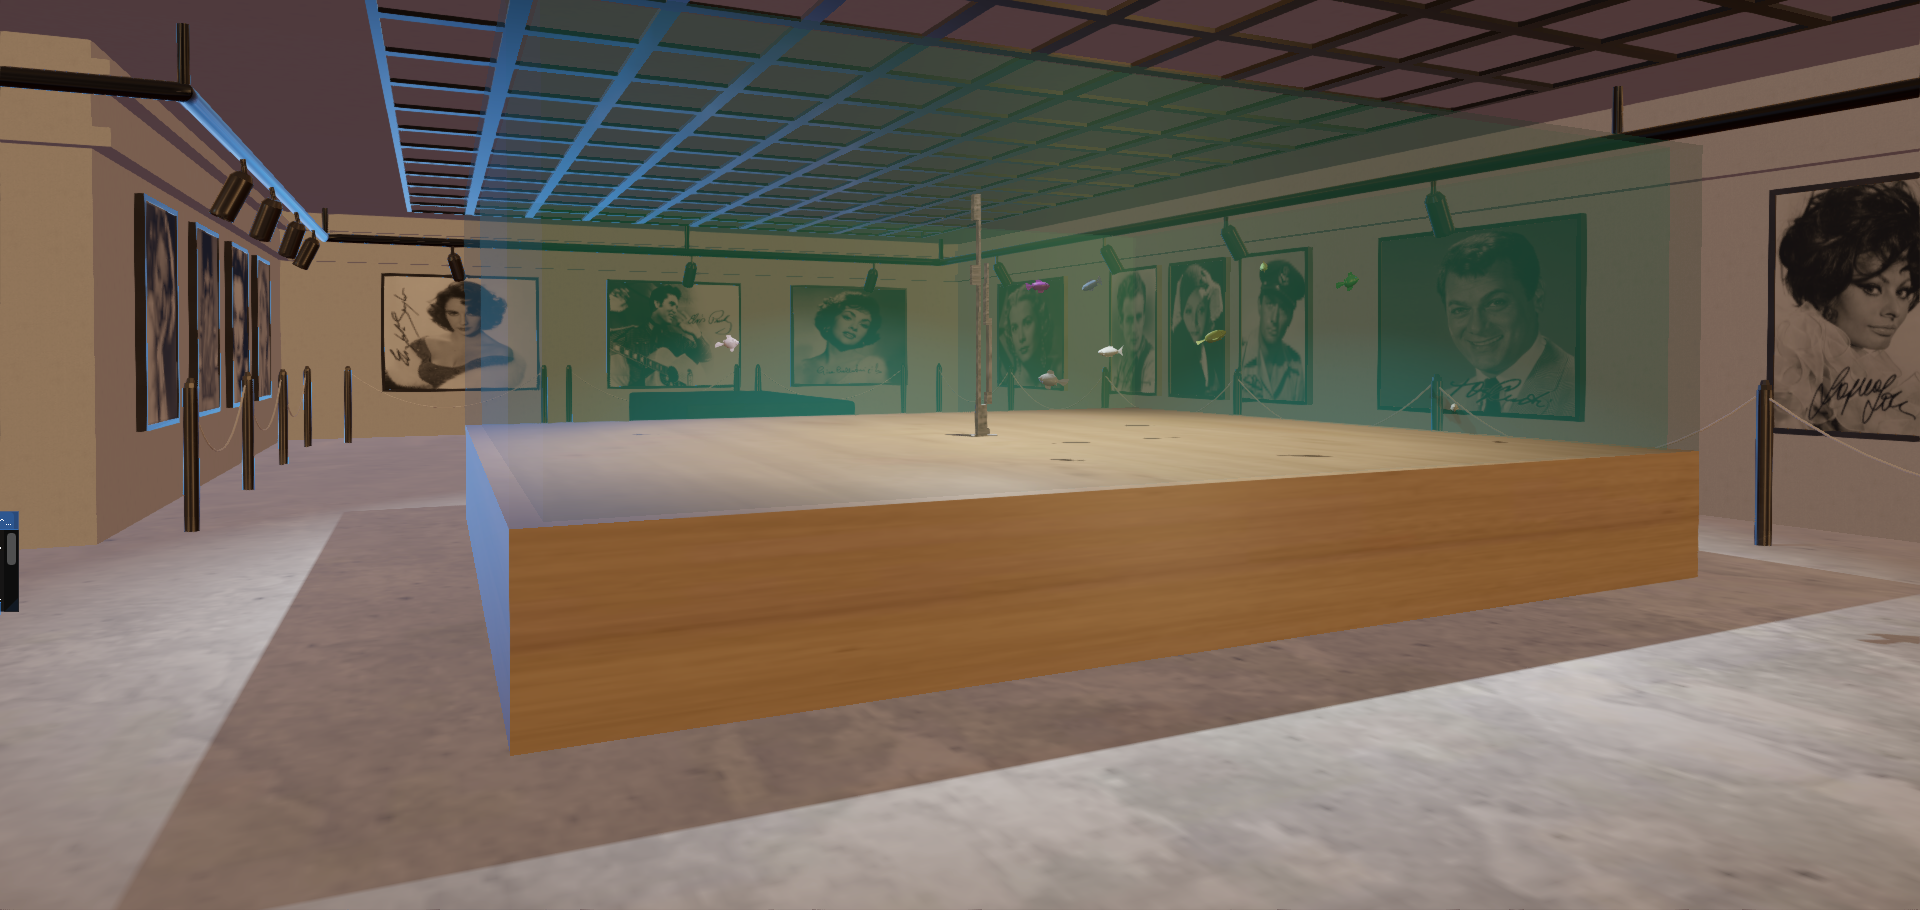
\includegraphics [scale=0.4] {my_folder/images//empty_aquarium}	
		\caption{Тестовая сцена. Количество рыб: 10} 
		\label{fig:empty_aquarium}
	\end{figure}
	
	\begin{figure}[ht!] 
		\center
		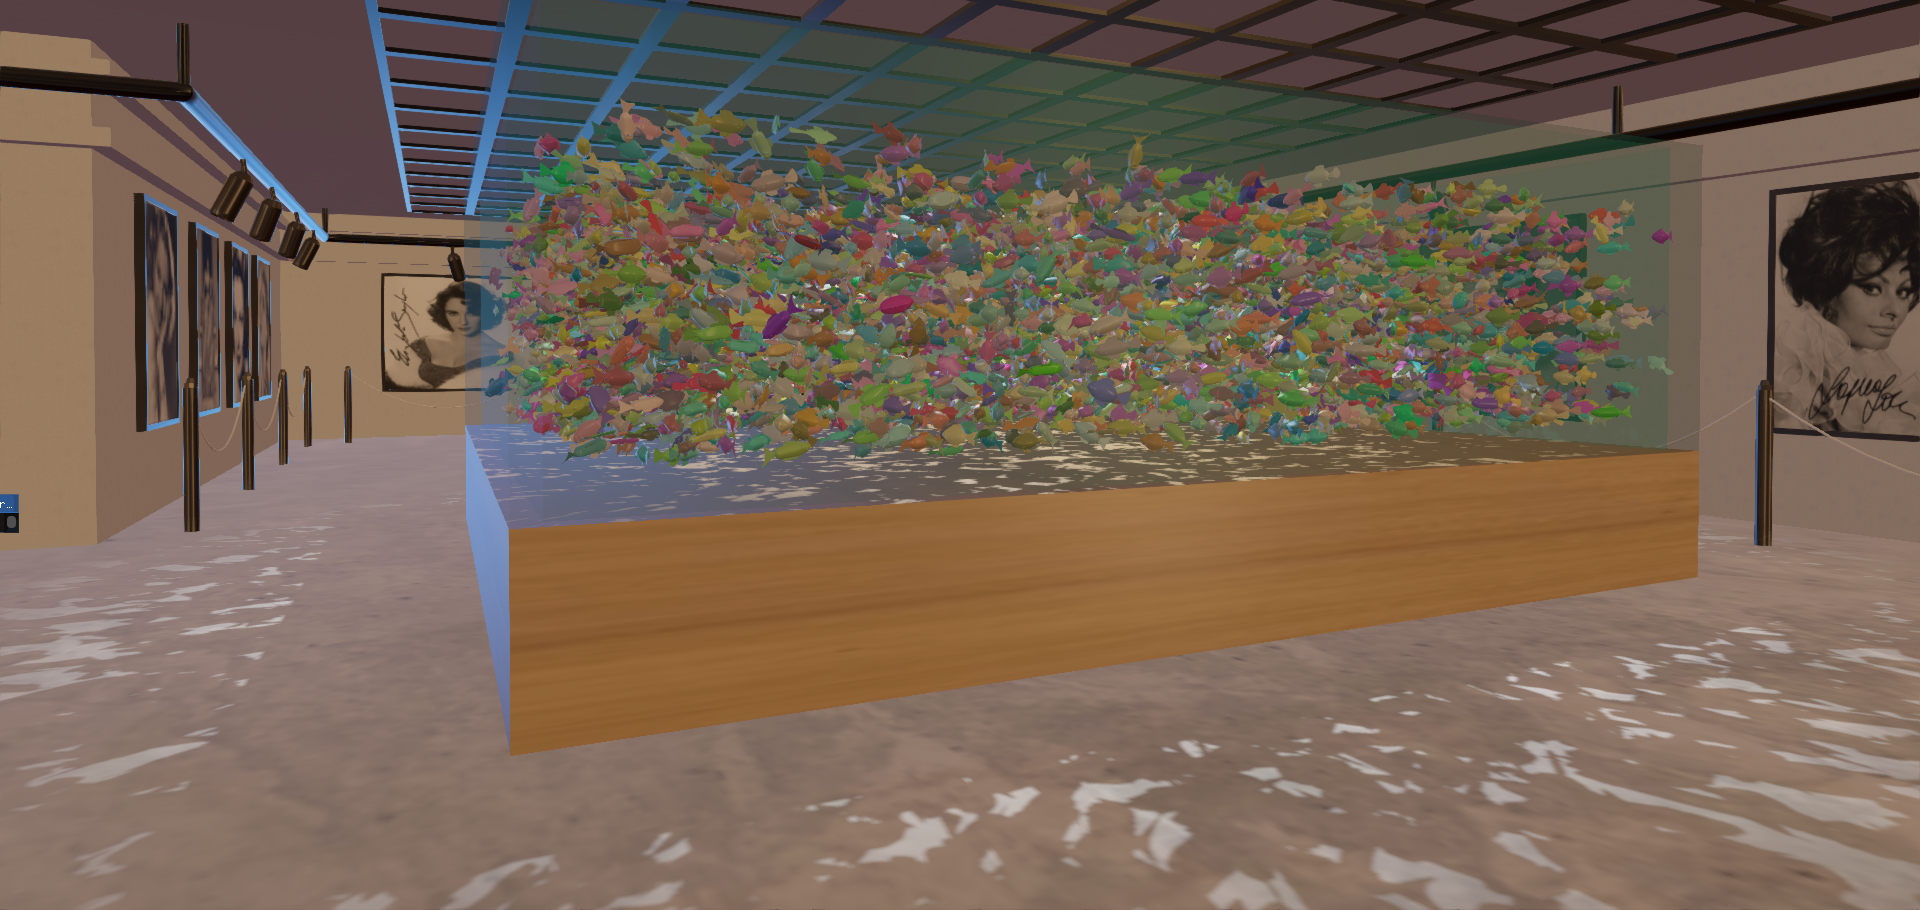
\includegraphics [scale=0.4] {my_folder/images//full_aquarium}	
		\caption{Тестовая сцена. Количество рыб: 8010} 
		\label{fig:full_aquarium}
	\end{figure}
	
	\FloatBarrier
	На данной сцене производились следующие измерения:
	\begin{enumerate}[1.]
		\item Зависимости количества кадров в секунду (FPS) от количества рыб
		\item Зависимости времени обработки кадра на графическом процессоре (GPU Time) от количества рыб
		\item Зависимости времени обработки кадра на центральном процессоре (CPU Time) от количества рыб
	\end{enumerate}

	Результаты представлены на графиках \firef{fig:fps_plot}, \firef{fig:gpu_plot} и \firef{fig:cpu_plot} соответственно. Значения \say{indirect} и соответствуют предлагаемой архитектуре, а значения \say{direct} соответствуют традиционной архитектуре. Эксперименты проводились на компьютере, с характеристиками представленными в таблице \ref{tab:spec}.
	
	\begin{table}[ht]
		\caption{Характеристики компьютера, на котором проводилось тестирование}
		\label{tab:spec}
		\centering
		\begin{SingleSpace}
			\begin{tabular}{|c|c|}
				\hline
				CPU & Intel Core 
				i5-9600K
				\\
				\hline
				GPU & nVidia RTX 2070 SUPER \\
				\hline
				RAM & 32 Gb \\
				\hline
		\end{tabular}
		\end{SingleSpace}
	\end{table}
	
	\begin{figure}[ht!] 
		\center
		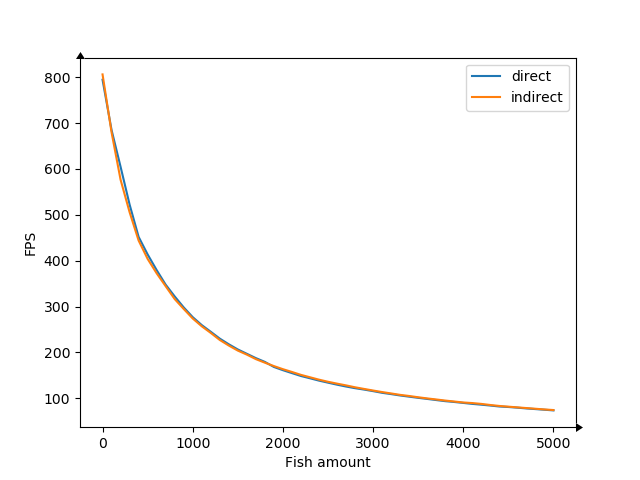
\includegraphics [scale=0.8] {my_folder/images//fps_plot}	
		\caption{График зависимости количества кадров в секунду (FPS) от количества рыб. } 
		\label{fig:fps_plot}
	\end{figure}

	\begin{figure}[ht!] 
		\center
		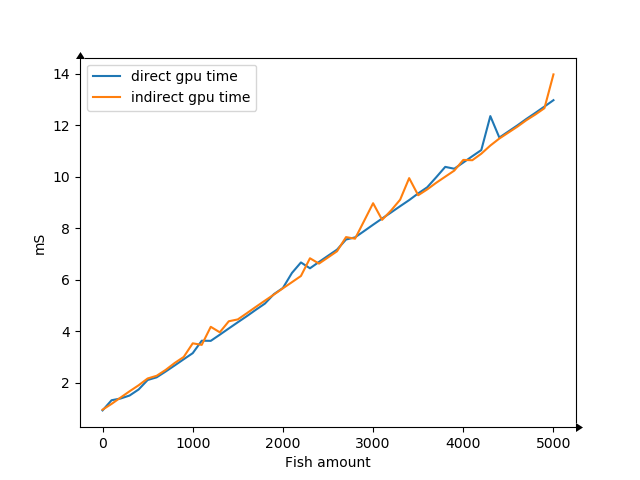
\includegraphics [scale=0.8] {my_folder/images//gpu_plot}	
		\caption{График зависимости времени обработки кадра на GPU (в миллисекундах) от количества рыб.} 
		\label{fig:gpu_plot}
	\end{figure}

	\begin{figure}[ht!] 
		\center
		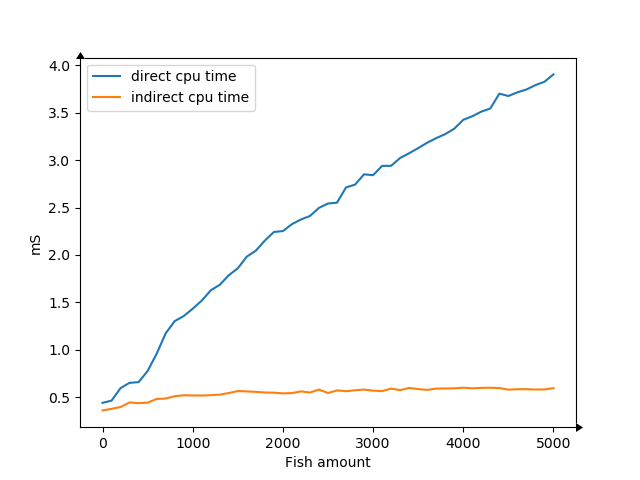
\includegraphics [scale=0.8] {my_folder/images//cpu_plot}	
		\caption{График зависимости времени обработки кадра на СPU (в миллисекундах) от количества рыб.} 
		\label{fig:cpu_plot}
	\end{figure}
	\FloatBarrier
	
	Как можно заметить по графикам \firef{fig:fps_plot} и \firef{fig:gpu_plot}, предлагаемая архитектура не вносит видимых изменений во время работы графического процессора. Однако, исходя из данных представленных на графике \firef{fig:cpu_plot} можно заметить, что предлагаемая архитектура требует гораздо меньше времени центрального процессора для построения кадра, чем традиционная. Таким образом, получившиеся экспериментальные результаты соответствуют теоритическим. 
	
	
%Хорошим стилем является наличие введения к главе. Во введении может быть описана цель написания главы, а также приведена краткая структура главы. 
	
%\section{Название параграфа} \label{ch4:sec1}

%\section{Название параграфа} \label{ch4:sec2}

%Пример ссылки на литературу \cite{avtonomova:fya,Peskov2004-ru,Kotelnikov2004-ru,Kotelnikov2004}.

%\FloatBarrier % заставить рисунки и другие подвижные (float) элементы остановиться

%\section{Выводы} \label{ch4:conclusion}

%Текст выводов по главе \thechapter.

%% Вспомогательные команды - Additional commands
%
%\newpage % принудительное начало с новой страницы, использовать только в конце раздела
%\clearpage % осуществляется пакетом <<placeins>> в пределах секций
%\newpage\leavevmode\thispagestyle{empty}\newpage % 100 % начало новой страницы